\documentclass[9pt,a4wide]{extarticle}

\usepackage{supertabular}
\usepackage[utf8]{inputenc}

\usepackage[scaled]{helvet}
\renewcommand\familydefault{\sfdefault} 
\usepackage[T1]{fontenc}

% \usepackage{german}
\usepackage{graphicx}
\usepackage{comment}
\usepackage{url}
\usepackage{multicol}

% toc linking does not work
%\usepackage{hyperref}
%\hypersetup{
%    colorlinks,
%    citecolor=black,
%    filecolor=black,
%    linkcolor=black,
%    urlcolor=black
%}

\parindent=0pt
\parskip=3pt
\topmargin 0cm

\textheight 22cm
\textwidth 17.5cm
\hoffset -3cm

\begin{document}

\begin{center}
{\LARGE\bf
     Python 3 Quick Reference\\
}
           \bigskip

          Hubert Högl

      Revision 0.5, 2019-01-24 
      
          2018, 2019

 \url{https://github.com/huberthoegl/pqr3}
      
\end{center}

\vskip 1cm

\newcommand{\rval}{$\rightarrow$\ }

\setlength{\columnsep}{2cm}
\begin{multicols}{2}
  \tableofcontents
\end{multicols}

\vfill

E-mail: {\tt <Hubert.Hoegl@t-online.de>}

This text ist licensed under the Creative Commons License CC-BY-NC-SA (please
see https://creativecommons.org).

\newpage

{\LARGE\bf ENVIRONMENT VARIABLES}
\addcontentsline{toc}{section}{Environment Variables}

PYTHONSTARTUP: file executed on interactive startup (no default)

PYTHONPATH: ':'-separated list of directories prefixed to the
 default module search path.  The result is sys.path.

PYTHONHOME: alternate <prefix> directory (or <prefix>:<exec\_prefix>).
 The default module search path uses <prefix>/pythonX.X.

PYTHONCASEOK: ignore case in 'import' statements (Windows).

PYTHONIOENCODING: Encoding[:errors] used for stdin/stdout/stderr.

PYTHONFAULTHANDLER: dump the Python traceback on fatal errors.

PYTHONHASHSEED: if this variable is set to
'random', a random value is used to seed the
hashes of str, bytes and datetime objects.  It
can also be set to an integer in the range
[0,4294967295] to get hash values with a
predictable seed.


\bigskip
{\LARGE\bf KEYWORDS}
\addcontentsline{toc}{section}{Keywords}

\begin{verbatim}
False      class      finally    is         return
None       continue   for        lambda     try
True       def        from       nonlocal   while
and        del        global     not        with
as         elif       if         or         yield
assert     else       import     pass
break      except     in         raise
\end{verbatim}




\bigskip
{\large\bf PYTHON}
\addcontentsline{toc}{section}{Python}

\begin{verbatim}
hhoegl@e11 ~$ python
Python 3.7.1 (default, Dec 14 2018, 19:28:38) 
[GCC 7.3.0] :: Anaconda, Inc. on linux
Type "help", "copyright", "credits" or "license" for more information.
>>> _ 
\end{verbatim}

\begin{itemize}
\item Basic Python prompt.
\item Tab Completion.
\item Use only for short "throw-away" interactive work.
\item For comfortable interactive work use {\tt IPython}.
\item Windows: Launcher {\tt py [Version] pgm.py}, newest Version default, 
      {\tt -2} for Python 2.
\end{itemize}


\bigskip
{\large\bf IPYTHON}
\addcontentsline{toc}{section}{IPython}

\begin{verbatim}
hhoegl@e11 ~$ ipython
Python 3.7.1 (default, Dec 14 2018, 19:28:38) 
Type 'copyright', 'credits' or 'license' for more information
IPython 7.2.0 -- An enhanced Interactive Python. Type '?' for help.
In [1]: _
\end{verbatim}

\bigskip

\begin{itemize}

\item Nice tab completion based on {\tt prompt\_toolkit} and {\tt ptpython}.

\item See page \pageref{ipy-section} for more information.

\end{itemize}



\bigskip
{\large\bf SOURCE ENCODING}
\addcontentsline{toc}{section}{Source Encoding}

\begin{itemize}

\item Default coding style for Python source files is {\tt UTF-8}. Use
    {\tt \# -*- coding: <encoding name> -*-} for alternate encodings.

\item Can use UTF-8 characters in strings, comments and identifiers:

\begin{verbatim}
         müll = "trööööt"    
\end{verbatim}
%  π = 3.141516
 
\item Unicode reader: [5] 

\end{itemize}

% TODO: Examples of IPython magic commands


\bigskip
{\LARGE\bf NUMBERS}
\addcontentsline{toc}{section}{Numbers}

Types: Integer, Float, Complex

Numbers are immutable

\begin{verbatim}
>>> i = 12
>>> j = -20
>>> u, v, w = 10, 12, 14

>>> p = 2 ** 100         # 2^100
>>> p
1267650600228229401496703205376

>>> f = 3.1415           # double (8 byte)

>>> 2.3 ** 100
1.4886191506362924e+36

>>> c = 4 + 3j           # complex number
\end{verbatim}



\medskip
{\bf Operations on Numbers}
\addcontentsline{toc}{subsection}{Operations on numbers}

\medskip

\begin{supertabular}{|l|p{12cm}|c|}\hline
{\em Operation}      & {\em Description}        &  {\em Notes} \\ \hline\hline

{\tt X + Y, X - Y}   & Add, subtract            &        \\ \hline
{\tt X * Y, X / Y}   & multiplication, division  &        \\ \hline
{\tt X // Y, X \% Y} & integer division, reminder  &        \\ \hline
{\tt -X, +X}         & sign                         &        \\ \hline
{\tt X | Y, X \& Y}   & bitwise or, bitwise and   &        \\ \hline
{\tt X \^{} Y}        &  exor                        &        \\ \hline
{\tt X << n, n >> n} &  shift                        &        \\ \hline
{\tt \~{}X}             & bitwise negate                      &        \\ \hline
{\tt X ** Y}         &  pow                        &        \\ \hline
{\tt abs(X)}         &  absolute value                        &        \\ \hline
{\tt int(X)}         &  type conversion                        &        \\ \hline
{\tt float(X)}         &  type conversion                        &        \\ \hline
{\tt complex(X)}         & type conversion        &        \\ \hline
{\tt divmod(X, Y)}       & integer division and reminder   &        \\ \hline
{\tt pow(X, Y, [Z])}     & identical with {\tt **}  &        \\ \hline
\end{supertabular}


\begin{itemize}
\item Also see modules {\tt decimal} (decimal floating point arithmetic) and
   {\tt fractions} (rational number arithmetic).
\end{itemize}


\bigskip
{\LARGE\bf Integer methods}
\addcontentsline{toc}{subsection}{Integer}

\begin{verbatim}
i.bit_length   i.denominator  i.imag         i.real         
i.conjugate    i.from_bytes   i.numerator    i.to_bytes    
\end{verbatim}

Example:

\begin{verbatim}
>>> i = 4 ** 100
>>> i.bit_length()
201
\end{verbatim}


\bigskip
{\LARGE\bf Float methods}
\addcontentsline{toc}{subsection}{Float}

\begin{verbatim}
f.as_integer_ratio  f.fromhex           f.imag              f.real              
f.conjugate         f.hex               f.is_integer        
\end{verbatim}



\bigskip
{\LARGE\bf Complex methods}
\addcontentsline{toc}{subsection}{Complex}

\begin{verbatim}
c.conjugate  c.imag       c.real
\end{verbatim}




\bigskip
{\LARGE\bf ASSIGNMENTS}
\addcontentsline{toc}{section}{Assignments}


\begin{verbatim}
a = 42              a **= b  
a += b              a &= b
a -= b              a |= b
a *= b              a ^= b
a /= b              a >>= b
a //= b             a <<= b
a %= b

a = 12 if cond else 0   # conditional expression
\end{verbatim}




\bigskip
{\LARGE\bf COMPARISONS}
\addcontentsline{toc}{section}{Comparisons}

\medskip

Comparisons are defined for any types.

\medskip

\begin{supertabular}{|l|p{12cm}|c|}\hline
{\em Operation}      & {\em Description}        &  {\em Notes} \\ \hline\hline

{\tt < }                   & less than                &        \\ \hline
{\tt <=}                   & less or equal            &        \\ \hline
{\tt > }                   & greater than             &        \\ \hline
{\tt >=}                   & greater or equal         &        \\ \hline
{\tt ==}                   & equal                    &        \\ \hline
{\tt !=}                   & not equal                &        \\ \hline
{\tt is}                   & identity                 &        \\ \hline
{\tt is not}               & negated identity         &        \\ \hline
\end{supertabular}

\medskip

\begin{itemize}
\item Works as expected: {\tt 0.2 <= f < 0.9}
\end{itemize}




\bigskip
{\LARGE\bf SEQUENCES, MAPPINGS and COLLECTIONS}
\addcontentsline{toc}{section}{Sequences, Mappings and Collections}

\begin{verbatim}
                   Sequences                         Mappings         Collections 
                /             \                         |               /      \
        immutable              mutable                mutable          mut    immut
       /    \      \           /     \                  |               |       |
 strings  bytes  tuples      list  bytearray           dict            set    frozenset


            INDEX: 0, 1, 2, 3, ...                  NO INDEX!!!
\end{verbatim}


Lit.: \url{https://docs.python.org/3/reference/datamodel.html}


\begin{verbatim}
Examples:

>>> s = "Hello World"
>>> B = bytes([3, 2, 9, 250])
>>> B[3]
250
>>> T = (7.32, "Hallo", 12)
>>> L = [3, "Hallo", 4.71, 2+5j]
>>> BA = bytearray([4, 9, 0, 255])
>>> BA[2] = 13
>>> D = { 0 : "Null", 1 : "Eins"}

>>> T = (1, 4, [4, 5, 9], 90)
>>> T[2][1] = 99

>>> b = True
>>> c = not True

>>> v = None
\end{verbatim}

\begin{itemize}
\item {\tt bytes()} $\rightarrow$ {\tt b'...'}
\end{itemize}




\bigskip
{\bf Operations on all sequences}
\addcontentsline{toc}{subsection}{Operations on all sequences}

\begin{supertabular}{|l|p{12cm}|c|}\hline
{\em Operation}      & {\em Description}        &  {\em Notes} \\ \hline\hline

{\tt len(S)}         & Number of elements in S  &        \\ \hline
{\tt x in S}         & x member in S            &        \\ \hline
{\tt x not in S}     & x not member in S        &        \\ \hline
{\tt S1 + S2}        & Concatenation                       &        \\ \hline
{\tt S * n}          & Sequence times int                  &        \\ \hline
{\tt n * S}          & Int times sequence                  &        \\ \hline
{\tt S[i]}           & Index Operator                      &        \\ \hline
{\tt S[i:j]}         & Slice Operator                      &        \\ \hline
{\tt S[i:j:k]}       & Slice Operator                      &        \\ \hline
{\tt S.index(x)}     & Get index of element x              &        \\ \hline
{\tt min(S)}         & Minimum                             &        \\ \hline
{\tt max(S)}         & Maximum                             &        \\ \hline
{\tt iter(S)}        & Return Iterator                     &        \\ \hline
{\tt for x in S:}    & Iteration                           &        \\ \hline
{\tt [e for e in S]} & List comprehension                  &        \\ \hline
{\tt map(f, S)}      & Functional programming              &        \\ \hline
{\tt filter(f, S)}   & Functional programming              &        \\ \hline
\end{supertabular}



\bigskip
{\bf Operations on mutable sequences}
\addcontentsline{toc}{subsection}{Operations on mutable sequences}

\begin{supertabular}{|l|p{12cm}|c|}\hline
{\em Operation }     &   {\em  Description}         & {\em  Notes} \\ \hline\hline

{\tt S[i] = x}       &   Assign x at index i in S   &        \\ \hline
{\tt S[i:j] = T}     &   Assign T to slice          &        \\ \hline
{\tt S[i:j:k] = T}   &   Assign T to slice          &        \\ \hline
{\tt del S[i]}       &   Delete                     &        \\ \hline
{\tt del S[i:j]}     &   Delete                     &        \\ \hline
{\tt del S[i:j:k]}   &   Delete                     &        \\ \hline
\end{supertabular}


\begin{itemize}
\item Change L {\em in place}: {\tt L[:] = [}{\em list compr. with L} {\tt ]}
\end{itemize}


\bigskip
{\bf Operations on Mappings}
\addcontentsline{toc}{subsection}{Operations on mappings}

\begin{supertabular}{|l|p{12cm}|c|}\hline
{\em Operation }     &   {\em  Description}         & {\em  Notes} \\ \hline\hline

{\tt D[k]}            &  Lookup dict by key k       &        \\ \hline
{\tt D[k] = x}        &  Key assignment             &        \\ \hline
{\tt del D[k]}        &  delete entry               &        \\ \hline
{\tt len(D)}          &  number of items in D       &        \\ \hline
{\tt k in D}          &  was {\tt D.has\_key(k)}    &        \\ \hline
{\tt k not in D}      &  test for key not in D      &        \\ \hline
{\tt iter(D)}         &  get iterator over keys ({\tt dict\_keyiterator})     &        \\ \hline
{\tt for k in D:}     &  iterate over keys          &        \\ \hline
\end{supertabular}


\bigskip
{\bf Operations on Sets}
\addcontentsline{toc}{subsection}{Operations on Sets}


\begin{supertabular}{|l|p{12cm}|c|}\hline
{\em Operation }     &   {\em  Description}             & {\em  Notes} \\ \hline\hline

{\tt len(S)}         & number of elements in S          &        \\ \hline
{\tt x in S}         & x is element of Set S            &        \\ \hline
{\tt S1 - S2}        & difference                       &        \\ \hline
{\tt S1 -= S2}       & difference update                &        \\ \hline
{\tt S1 | S2}        & union                            &        \\ \hline
{\tt S1 |= S2}       & union update                     &        \\ \hline
{\tt S1 \& S2}       & intersection                     &        \\ \hline
{\tt S1 \^{} S2}     & symmetric difference             &        \\ \hline
{\tt S1 \^{}= S2}    & symmetric difference update      &        \\ \hline
{\tt S1 < S2}        & test for true subset             &        \\ \hline
{\tt S1 <= S2}       & test for subset                  &        \\ \hline
{\tt S1 > S2}        & test for true superset           &        \\ \hline
{\tt S1 >= S2}       & test for superset                &        \\ \hline
{\tt S1 != S2}       & test for unequal sets            &        \\ \hline

\end{supertabular}

\medskip

See also section SET METHODS below.


\bigskip
{\LARGE\bf STRING METHODS}
\addcontentsline{toc}{section}{String Methods}

IPython Hilfe ({\tt s.<tab>})

\begin{verbatim}
s.capitalize    s.format        s.islower       s.lower         s.rpartition    s.title
s.casefold      s.format_map    s.isnumeric     s.lstrip        s.rsplit        s.translate
s.center        s.index         s.isprintable   s.maketrans     s.rstrip        s.upper
s.count         s.isalnum       s.isspace       s.partition     s.split         s.zfill
s.encode        s.isalpha       s.istitle       s.replace       s.splitlines    
s.endswith      s.isdecimal     s.isupper       s.rfind         s.startswith    
s.expandtabs    s.isdigit       s.join          s.rindex        s.strip         
s.find          s.isidentifier  s.ljust         s.rjust         s.swapcase     
\end{verbatim}


\begin{supertabular}{|l|p{9cm}|c|}\hline
{\em Method}            & {\em Description}                    &  {\em Notes} \\ \hline\hline

{\tt s.capitalize() }   &    Returns a copy of s with its first character capitalized, and the rest of the characters lowercase.   &        \\ \hline

{\tt s.casefold() }   &  Return a version of s suitable for caseless comparisons. &   \\ \hline 
{\tt s.center(width[, fillchar])} &    
Returns a copy of s centered in a string of length {\em width}, surrounded by the appropriate number of {\em fillchar} characters.  &
    \\ \hline

{\tt s.count(sub[, start[, end]])}   &  Return number of non-overlapping occurrences of substring sub in string s[start:end].  Optional arguments start and end are interpreted as in slice notation.  &        \\ \hline

{\tt s.encode([encoding [, errors]]) }  & Encode s using the codec registered for encoding. Return {\tt bytes}.   &    \\ \hline

{\tt s.endswith(suffix [,start [,end]]) }  & Return True if s ends with the specified suffix, False otherwise. &        \\ \hline

{\tt s.expandtabs([tabsize]) }  &  Return a copy of s where all tab characters are expanded using spaces.  If tabsize is not given, a tab size of 8 characters is assumed.
&        \\ \hline

{\tt s.find(sub [,start [,end]]) }   &  Return the lowest index in s where substring sub is found, such that sub is contained within s[start:end].  Optional
arguments start and end are interpreted as in slice notation.&        \\ \hline

{\tt s.format(*args, **kwargs) }   &  see \url{https://pyformat.info}               &        \\ \hline

{\tt s.format\_map(mapping) }   & Return a formatted version of s, using substitutions from mapping.  &        \\ \hline

{\tt s.index(sub [,start [,end]]) }   &   Like s.find() but raise ValueError when the substring is not found.   &        \\ \hline

{\tt s.isalnum() }   &   Return True if all characters in s are alphanumeric
and there is at least one character in s, False otherwise.&        \\ \hline

{\tt s.isalpha() }   &  Return True if all characters in s are alphabetic
and there is at least one character in s, False otherwise.&        \\ \hline

{\tt s.isdecimal() }   &  Return True if there are only decimal characters in s,
False otherwise.
&        \\ \hline

{\tt s.isdigit() }   &  Return True if all characters in s are digits
and there is at least one character in s, False otherwise.  &        \\ \hline

{\tt s.isidentifier() }   &  Return True if s is a valid identifier according
to the language definition.  &        \\ \hline

{\tt s.islower() }   &  Return True if all cased characters in s are lowercase and there is at least one cased character in s, False otherwise.&        \\ \hline

{\tt s.isnumeric() }   &   Return True if there are only numeric characters in s, False otherwise.&        \\ \hline

{\tt s.isprintable() }   &  Return True if all characters in s are considered
printable in repr() or s is empty, False otherwise.&        \\ \hline

{\tt s.isspace() }   &  Return True if all characters in s are whitespace
and there is at least one character in s, False otherwise.&        \\ \hline

{\tt s.istitle() }   & Return True if s is a titlecased string  &        \\ \hline

{\tt s.isupper() }   &  Return True if all cased characters in s are uppercase and there is at least one cased character in s, False otherwise. &        \\ \hline

{\tt s.join(iterable) }   & Return a string which is the concatenation of the strings in the
iterable.  The separator between elements is s.&        \\ \hline

{\tt s.ljust(width [,fillchar]) }  &  Return s left-justified in a Unicode string of length width. Padding is done using the specified fill character (default is a space).&        \\ \hline

{\tt s.lower() }   &  Return a copy of the string s converted to lowercase.    &        \\ \hline

{\tt s.lstrip([chars]) }   &  Return a copy of the string s with leading whitespace removed.  If chars is given and not None, remove characters in chars instead.&        \\ \hline

{\tt s.maketrans() }   & Return a translation table usable for {\tt s.translate()}.     &        \\ \hline

{\tt s.partition(sep) }   &  \rval (head, sep, tail).  Search for the separator sep in s, and return the part before it, the separator itself, and the part after it.  If the separator is not found, return s and two empty strings.&        \\ \hline

{\tt s.replace(old, new [,count]) }   &  Return a copy of s with all occurrences of substring old replaced by new.  If the optional argument count is given, only the first count occurrences are replaced.  &        \\ \hline

{\tt s.rfind(sub [,start [,len]]) }   &  Return highest index in s where substring sub is found, such that sub is contained within s[start:end].&     \\ \hline

{\tt s.rindex(sub [,start [,len]]) }   &  Like s.rfind() but raise ValueError when the substring is not found.         &        \\ \hline

{\tt s.rjust(width [,fillchar]) }   &  Return s right-justified in a string of length width. Padding is done using the specified fill character (default is a space).&        \\ \hline

{\tt s.rpartition(sep) }   & Search for the separator sep in s, starting at the
end of s, and return the part before it, the separator itself, and the part
after it.  If the separator is not found, return two empty strings and s. & \\ \hline

{\tt s.rsplit([sep [,maxsplit]]) }   &  \rval list of strings. Return a list of the words in s, using sep as the delimiter string, starting at the end of the string and working to the front.  If maxsplit is given, at most maxsplit splits are done. If sep is not specified, any whitespace string is a separator.&        \\ \hline

{\tt s.rstrip([chars]) }   & Return a copy of the string s with trailing whitespace removed.  If chars is given and not None, remove characters in chars instead.&        \\ \hline

{\tt s.split([sep [,maxsplit]]) }   & \rval list of strings. Return a list of the words in s, using sep as the delimiter string.  If maxsplit is given, at most maxsplit splits are done. If sep is not specified or is None, any whitespace string is a separator and empty strings are removed from the result.&        \\ \hline

{\tt s.splitlines([keepends]) }   &  \rval list of strings. Return a list of the lines in s, breaking at line boundaries.  Line breaks are not included in the resulting list unless keepends is given and true. &        \\ \hline

{\tt s.startswith(prefix [,start [,end]]) }  & Return True if s starts with the specified prefix, False otherwise.  With optional start, test s beginning at that position.  With optional end, stop comparing s at that position.  prefix can also be a tuple of strings to try.  &        \\ \hline

{\tt s.strip([chars]) }   &  Return a copy of the string s with leading and trailing whitespace removed.&        \\ \hline

{\tt s.swapcase() }   & Return a copy of s with uppercase characters converted to lowercase and vice versa. &  \\ \hline

{\tt s.title() }   &  Return a titlecased version of s   &        \\ \hline

{\tt s.translate(table [,deletechars]) }   & Return a copy of the string s in which each character has been mapped through the given translation table. \dots{} &        \\ \hline

{\tt s.upper() }   & Return a copy of s converted to uppercase   &        \\ \hline

{\tt s.zfill(width) }   & \rval str. Pad a numeric string s with zeros on the left, to fill a field of the specified width. The string s is never truncated. &   \\ \hline

\end{supertabular}

\medskip

\begin{itemize}
\item String concatenation: {\tt 'abc' 'def' 'ghi'}
\end{itemize}




\bigskip
{\LARGE\bf TUPLE METHODS}
\addcontentsline{toc}{section}{Tuple Methods}

\begin{verbatim}
T.count  T.index 
\end{verbatim}

\begin{supertabular}{|l|p{9cm}|c|}\hline
{\em Method}  & {\em Description}     &  {\em Notes}       \\ \hline\hline

{\tt T.count(value)}  &  return number of occurrences of value          &                \\ \hline

{\tt T.index(value, [start, [stop]])}  &  Return first index of value   &    \\ \hline

\end{supertabular}

\bigskip

Also see section {\em Operations on all sequences}

\medskip

Examples:

\begin{verbatim}
>>> T = (3, 5, 1, 20, 4)
>>> len(T)
5
>>> T[1:-1]
(5, 1, 20)
>>> a, *b, c = T
>>> a, b, c
(3, [5, 1, 20], 4)
\end{verbatim}



\bigskip
{\LARGE\bf LIST METHODS}
\addcontentsline{toc}{section}{List Methods}

% IPython: {\tt L.<tab>}

\begin{verbatim}
L.append*   L.copy     L.extend*   L.insert*   L.remove*    L.sort*    
L.clear*    L.count    L.index     L.pop*      L.reverse* 
\end{verbatim}

Operations marked with {\tt *} are in-place.

\bigskip

\begin{supertabular}{|l|p{9cm}|c|}\hline
{\em Method}  & {\em Description}       &    {\em Notes}   \\ \hline\hline

{\tt L.append(obj)}  & \rval None. Append obj to end.          &          \\ \hline

{\tt L.clear()}  &  \rval None. Remove all items from L.     &      \\ \hline

{\tt L.copy()}  &  Return a shallow copy of L.         &     \\ \hline

{\tt L.count(value)}  &  Return number of occurrences of value. &           \\ \hline

{\tt L.extend(iterable)}  &  \rval None. Extend list by appending elements from the iterable.    &        \\ \hline

{\tt L.index(value, [start, [stop]])}  &  Return first index of value.     &       \\ \hline

{\tt L.insert(index, object)}  &  \rval None. Insert object before index.    &     \\ \hline

{\tt L.pop([index])}  &  Remove and return item at index (default last).  & \\ \hline 

{\tt L.remove(value)}  &  \rval None. Remove first occurrence of value.                       &    \\ \hline

{\tt L.reverse()}  & \rval None. Reverse in-place.    &     \\ \hline

{\tt L.sort(key=None, reverse=False)}  & \rval None. Sort in-place.          &    \\ \hline

\end{supertabular}

\medskip

\begin{itemize}

\item List Comprehension

     \begin{verbatim}
     L = [e**2 for e in range(10)]

     L[:] = [e**2 for e in L]       # change L in place
     \end{verbatim}

\end{itemize}


Examples:

\begin{verbatim}
>>> L = [23, 2, 9, 7, 13]
>>> M = L                 # two references to same object
>>> L[1] = 99
>>> M[1]
99                        # !!!
>>> K = L[:]              # two references to different objects
>>> K[1] = 5
>>> L[1]                    
99
\end{verbatim}




\bigskip
{\LARGE\bf DICTIONARY METHODS}
\addcontentsline{toc}{section}{Dictionary Methods}

\begin{verbatim}
D.clear*      D.fromkeys    D.items       D.pop         D.setdefault  D.values      
D.copy        D.get         D.keys        D.popitem     D.update* 
\end{verbatim}

\bigskip

\begin{supertabular}{|l|p{9cm}|c|}\hline
{\em Method}  & {\em Description}   &  {\em Notes}         \\ \hline\hline

{\tt D.clear()}  & Remove all items from D; \rval None  &  \\ \hline

{\tt D.copy()}  & Return a shallow copy of D   &  \\ \hline
    
{\tt D.fromkeys(iterable [,value])}  &  Return a new dictionary with keys from a supplied iterable and values all set to specified value (default None).  &  \\ \hline 

{\tt D.get(k [,d])}  & Return D[k] if k in D, else d; d defaults to None. &  \\ \hline

{\tt D.items()}  &  Return a set-like object providing a view on D's items  &  \\ \hline

{\tt D.keys()}  &  Return a set-like object providing a view on D's keys  &   \\ \hline

{\tt D.pop(k [,d])}  &  Remove given key k, Return corresponding value. If key not found \rval d if given; else KeyError. &   \\ \hline

{\tt D.popitem()}  &  Remove and return some (key, value) pair  &   \\ \hline 


{\tt D.setdefault(k [,d])}  & D.get(k,d), also set D[k]=d if k not in D   &   \\ \hline

{\tt D.update([E, ]**F)}  & Update D from dict/iterable E and F; \rval None   &   \\ \hline 

{\tt D.values()}  &  Return an object providing a view on D's values   &    \\ \hline 
\end{supertabular}

\bigskip

Examples

\begin{verbatim}
>>> D = {0: "Null", 1: "Eins"}
>>> v = D.keys()   # v is a "view"
>>> v
dict_keys([0, 1])
>>> for k in v:
>>>     print(k)
>>> D.values()
dict_values(['Null', 'Eins'])
>>> it = D.items()
>>> it
dict_items([(0, 'Null'), (1, 'Eins')])
>>> for k, v in it:
>>>    print(k, v)
>>> E = { "Hans" : 1234, "Maria" : 4321 }
>>> D.update(E, Thorsten=7890)
\end{verbatim}

\begin{itemize}
\item D.keys(), D.values(), D.items() return {\em views}. 
\item Sort a view with {\tt sorted()}.
\item Dictionary comprehension
\end{itemize}




\bigskip
{\LARGE\bf SET METHODS}
\addcontentsline{toc}{section}{Set Methods}

\begin{verbatim}
s.add                          s.intersection (&)             s.remove
s.clear                        s.intersection_update (s &= t) s.symmetric_difference (^)
s.copy                         s.isdisjoint                   s.symmetric_difference_update (^=)
s.difference (-)               s.issubset (<=)                s.union (|)
s.difference_update (-=)       s.issuperset (>=)              s.update (|=)
s.discard                      s.pop                          
\end{verbatim}


\bigskip

\begin{supertabular}{|l|p{11cm}|c|}\hline
{\em Method}  & {\em Description}            \\ \hline\hline

{\tt s.add(x)}  & Add an element to S; do nothing if element exists in S  \\ \hline
{\tt s.clear()}  & Remove all elements from S  \\ \hline
{\tt s.copy()}  &  \rval a new set with a shallow copy of s.  \\ \hline
{\tt s.difference(t, ...)}  & \rval new set with elements in the set that are not in the others.  \\ \hline
{\tt s.difference\_update(t, ...)}  & Update the set, removing elements found in others  ({\tt s -= t})                             \\ \hline
{\tt s.discard(elem)}  & Remove elem in set s if present.  \\ \hline
{\tt s.intersection(t, ...)}  & \rval a new set with elements common to the set and all others ({\tt s \& t})          \\ \hline
{\tt s.intersection\_udate(t)}  & \rval set s keeping only elements also found in t ({\tt s \&= t})  \\ \hline
{\tt s.disjoint(t)}  & \rval True if the set has no elements in common with t. Sets are disjoint if and only if their intersection is the empty set.   \\ \hline
{\tt s.issubset(t)}  & Test whether every element in the set is in t ({\tt <=}).  \\ \hline
{\tt s.issuperset(t)}  & Test whether every element in t is in the set ({\tt >=}) \\ \hline
{\tt s.pop()}  & Remove and return an arbitrary element from the set. Raises KeyError if the set is empty.  \\ \hline
{\tt s.remove(e)}  & Remove element e from the set. Raises KeyError if 
elem is not contained in the set.  \\ \hline
{\tt s.symmetric\_difference(t)}  &  \rval a new set with elements in either the set or other but not both ({\tt s \^{} t})   \\ \hline
{\tt s.symmetric\_difference\_update(t)}  & Update the set, keeping only elements found in either set, but not in both ({\tt s \^{}= t})    \\ \hline
{\tt s.union(t, ...)}  & Return a new set with elements from the set and all others ({\tt |}).  \\ \hline
{\tt s.update(t, ...)}  & Update the set, adding elements from all others ({\tt |=})   \\ \hline
\end{supertabular}

\bigskip

Example:

\begin{verbatim}
>>> T = {"e", "a", "g"}        # {} is a dict. Use set() for empty set.
>>> S = set(["a", "b", "c"])   
>>> S - T 
{'b', 'c'}
>>> S | T
{'a', 'b', 'c', 'e', 'g'}
\end{verbatim}

\begin{itemize}
\item {\tt a < b} $\rightarrow$ {\tt a <= b and a != b}
\item Set comprehensions
\item {\tt frozenset()}
\end{itemize}




\bigskip
{\LARGE\bf FUNCTIONS}
\addcontentsline{toc}{section}{Functions}

\begin{itemize}

\item 

   \begin{verbatim}
   def f1(a, b, c):
       return [a, b, c]

   f1(2, 5, 9)
   \end{verbatim}

\item

   \begin{verbatim}
   def f2(a, b=5, c=9):
       return [a, b, c]

   f1(2)
   f1(2, 5, 9)
   f1(2, c=3)
   f1(2, b=7)
   f1(2, c=3, b=4)
   \end{verbatim}

\item 

   \begin{verbatim}
   def f3(a, b, c=5, d=9):                 def f3(*posargs, **kwargs):
       return (a, b), {'c':c, 'd':d}           return posargs, kwargs

                         T = (3, 7)
                         D = { 'c': 14, 'd': 23 }
                         f3(*T, **D}
   \end{verbatim}

\item 

   \begin{verbatim}
   def f4():
       return 'a', 'b', 'c', 'd', 'e'

   m, *n, o = f4()
   \end{verbatim}

\end{itemize}



\bigskip
{\LARGE\bf BUILTIN FUNCTIONS}
\addcontentsline{toc}{section}{Builtin Functions}

\begin{verbatim}
abs()           dict()        help()          min()         setattr()
all()           dir()         hex()           next()        slice()
any()           divmod()      id()            object()      sorted()
ascii()         enumerate()   input()         oct()         staticmethod()
bin()           eval()        int()           open()        str()
bool()          exec()        isinstance()    ord()         sum()
bytearray()     filter()      issubclass()    pow()         super()
bytes()         float()       iter()          print()       tuple()
callable()      format()      len()           property()    type()
chr()           frozenset()   list()          range()       vars()
classmethod()   getattr()     locals()        repr()        zip()
compile()       globals()     map()           reversed()  
complex()       hasattr()     max()           round() 
delattr()       hash()        memoryview()    set() 
\end{verbatim}

\bigskip

\begin{supertabular}{|l|p{9.5cm}|c|}\hline
{\em Method}  & {\em Description}            \\ \hline\hline

{\tt abs(x)}  &  Returns the absolute value of the number x     \\ \hline

{\tt all(iter)}   &  Return True if all elements of the iterable are true (or if the iterable is empty) \\ \hline

{\tt any(iter)} & Return True if any element of the iterable is true.\\ \hline 

{\tt ascii(obj)}  &  Return a repr string with non-ASCII escaped  \\ \hline

{\tt bin(x)}   &  Convert integer number to binary string  \\ \hline

{\tt bool([x])}   & \rval True when the argument x is true, False otherwise \\ \hline

{\tt bytearray([arg [,encoding [,errors]]])}  &  Construct an mutable bytearray object from iterable-of-ints/str/bytes-of-buffer/int  \\ \hline

{\tt bytes([arg [,encoding [,errors]]])} & Construct an immutable array of bytes   \\ \hline

{\tt callable(obj)}   & \rval whether obj is callable (bool)   \\ \hline

{\tt chr(i)}       &  \rval a Unicode string of one character with ordinal i; 0 <= i <= 0x10ffff.     \\ \hline

{\tt classmethod(fn)}  & \rval method; Convert a function to be a class method.
\\ \hline

{\tt compile(source, filename, mode)}  &  Compile the source (a Python 
module, statement or expression) into a code object that can be executed 
by exec() or eval().  \\ \hline

{\tt complex(real [,imag])} &                                  \\ \hline

{\tt delattr(obj, name)}  & Delete a named attribute on an object; 
   delattr(x, 'y') is equivalent to "del x.y".\\ \hline

{\tt dict([arg])}       &                                         \\ \hline

{\tt dir([object])}       &   If called without an argument, return the names
in the current scope.  Else, return an alphabetized list of names comprising
(some of) the attributes of the given object, and of attributes reachable from
it.  If the object supplies a method named {\tt \_\_dir\_\_}, it will be used;
otherwise the default {\tt dir()} logic is used and returns: For a module
object: the module's attributes.  For a class object:  its attributes, and
recursively the attributes of its bases.  For any other object: its attributes,
its class's attributes, and recursively the attributes of its class's base
classes.  \\ \hline

{\tt divmod(x, y)}       & \rval (div, mod); this is the tuple 

{\tt ((x-x\%y)/y, x\%y)}  \\ \hline

{\tt enumerate(iter, start=0)} & \rval enumerate object which yields pairs 
containing a count  and a value yielded by the iterable argument:
{\tt (0, seq[0]), (1, seq[1]), (2, seq[2]), ...}\\ \hline

{\tt eval(source [,globals [,locals]])} &  Evaluate the source in the context
of globals and locals.  The source may be a string representing a Python
expression or a code object as returned by compile().  \\ \hline

{\tt exec(object[, globals[, locals]])} & Read and execute code from an object,
which can be a string or a code object.  The globals and locals are
dictionaries, defaulting to the current globals and locals.  If only globals is
given, locals defaults to it.\\ \hline

{\tt filter(fn, iter)} & \rval an iterator yielding those items of iterable
for which function(item) is true. If function is None, return the items that
    are true.\\ \hline

{\tt float([x])}  &  Convert a string or number to a floating point number, if
possible.  \\ \hline

{\tt format(value [,format\_spec])}  & \rval formatted string  \\ \hline

{\tt frozenset([iter])}  &  Build an immutable unordered collection of unique elements.  \\ \hline

{\tt getattr(obj, name [,default])}  & Get a named attribute from an object;
getattr(x, 'y') is equivalent to x.y.  When a default argument is given, it is
returned when the attribute doesn't exist; without it, an exception is raised
in that case.\\ \hline

{\tt globals()} & \rval the dictionary containing the current scope's global
variables.  \\ \hline

{\tt hasattr(obj, name)} &  \rval whether the object has an attribute with the given name.  \\ \hline

{\tt hash(obj)}  &  \rval an (int) hash value for the object. \\ \hline 

{\tt help([obj])}  &  This is a wrapper around pydoc.help that provides a helpful message when 'help' is typed at the Python interactive prompt. \\ \hline

{\tt hex(x)} &                                      \\ \hline

{\tt id(obj)} & \rval identity of an object (int). This is guaranteed to be unique among simultaneously existing objects.\\ \hline

{\tt input([prompt])} & Read a string from standard input.  The trailing
newline is stripped.  If the user hits EOF (Unix: Ctl-D, Windows:
Ctl-Z+Return), raise EOFError.  On Unix, GNU readline is used if enabled.  The
prompt string, if given, is printed without a trailing newline before reading.
\\ \hline

{\tt int([number | string [,base])}  & Convert a number or string to an
integer, or return 0 if no arguments are given.  If x is a number, return
{\tt x.\_\_int\_\_()}.  For floating point numbers, this truncates towards zero.
\\ \hline

{\tt isinstance(obj, class-or-type-or-tuple)}  & Return whether an object is an instance of a class or of a subclass thereof.  \\ \hline

{\tt issubclass(C, B)}  & Return whether class C is a subclass (i.e., a derived class) of class B. \\ \hline

{\tt iter(iterable)}  & Get an iterator from an object. The argument must 
supply its own iterator, or be a sequence. \\ \hline 

{\tt iter(callable, sentinel)}  & Get an iterator from a callable. The 
callable is called until it returns the sentinel.  \\ \hline

{\tt len(obj)}  & \rval number of items of a sequence or collection. \\ \hline

{\tt list([iter])}  & \rval new list initialized from iterable's items \\ \hline

{\tt locals()}  &  Update and return a dictionary containing the current 
   scope's local variables.   \\ \hline

{\tt map(func, *iterables)} & \rval map object; Make an iterator that computes
the function using arguments from each of the iterables.  Stops when the
shortest iterable is exhausted.  \\ \hline

{\tt max(iterable, *[, default=obj, key=func])} &  With a single iterable
argument, return its biggest item. The default keyword-only argument specifies
an object to return if the provided iterable is empty.  
\\ \hline

{\tt max(arg1, arg2, *args, *[, key=func]) } & With two or more
arguments, return the largest argument. \\ \hline 

{\tt memoryview(obj)} & Create a new memoryview object which references the given object.  \\ \hline

{\tt min(iterable, *[, default=obj, key=func])}  & \rval smallest argument  \\ \hline

{\tt next(iter [,default])} &  \rval next item from the iterator. If
default is given and the iterator is exhausted, it is returned instead of
raising StopIteration.  \\ \hline

{\tt object()} & \rval new featureless object. object is a base for all classes. \\ \hline

{\tt oct(number)} & \rval octal representation of an integer. \\ \hline

{\tt open(file, **kwargs)} &  Open file and return a stream (file object). Raise IOError upon failure. 

     \smallskip

{\tt open(file, mode='r', buffering=-1, encoding=None, errors=None, newline=None, closefd=True, opener=None)} \\ \hline

{\tt ord(c)} & \rval octal representation of an integer \\ \hline

{\tt pow(x, y [,z])} &  With two arguments, equivalent to {\tt x**y}.  With
three arguments, equivalent to {\tt (x**y) \% z}, but may be more efficient
(e.g. for ints).
\\ \hline

{\tt print(obj, ..., sep, end, file, flush)}   & Prints the values to a stream, or to sys.stdout by default.  \\ \hline

{\tt property(**kwargs)}  & Define managed attributes. See also decorator
  {\tt @property} \\ \hline

{\tt range(stop)} & \rval sequence of numbers from 0 to stop - 1 \\ \hline

{\tt range(start, stop [,step])} & \rval sequence of numbers from start to stop - 1 by step.  \\ \hline

{\tt repr(obj)}  & \rval canonical string representation of the object. For
 most objects {\tt eval(repr(object)) == object} \\ \hline

{\tt reversed(sequence)}  &  \rval reverse iterator   \\ \hline 

{\tt round(x [,ndigits])}  & Round a number to a given precision in decimal
digits (default 0 digits).  This returns an int when called with one argument,
otherwise the same type as the number. ndigits may be negative.\\ \hline

{\tt set(iter)}  &  Build an unordered collection of unique elements. \\ \hline 

{\tt setattr(obj, name, val)}  &  Set a named attribute on an object; 
   setattr(x, 'y', v) is equivalent to x.y = v.                 \\ \hline

{\tt slice(start, stop [,step])} & Create a slice object. This is used for 
extended slicing (e.g. a[0:10:2]).   \\ \hline

{\tt sorted(iterable, key=None, reverse=False)} &  \rval new sorted list  \\ \hline

{\tt staticmethod(function)}  & Convert a function to be a static method \\ \hline

{\tt str([bytes-or-buffer ,[enc [,err]]])} & Create a new string object from
the given object. If encoding or errors is specified, then the object must
expose a data buffer that will be decoded using the given encoding and error
handler.  Otherwise, returns the result of object.\_\_str\_\_() (if defined)
or repr(object).  \\ \hline

{\tt sum(iter [,start])} &  \rval sum of an iterable of numbers (NOT
strings) plus the value of parameter 'start' (which defaults to 0).  When the 
iterable is empty, return start.  \\ \hline

{\tt super([type [,obj-or-type]])}       &                      \\ \hline

{\tt tuple([iter])} & \rval tuple initialized from iterable's items \\ \hline 

{\tt type(obj)}     & \rval the obj's type         \\ \hline

{\tt vars([obj])}   & \rval dictionary; Without arguments, equivalent to 
locals().  With an argument, equivalent to {\tt object.\_\_dict\_\_}.
\\ \hline

{\tt zip(*iters)}   & \rval a zip object whose {\tt .\_\_next\_\_()}
method returns a tuple where the i-th element comes from the i-th iterable
argument.  The {\tt .\_\_next\_\_()} method continues until the shortest
iterable in the argument sequence is exhausted and then it raises
StopIteration.  \\ \hline

\end{supertabular}


\bigskip

Lit.: 

\begin{itemize} 

\item IPython magic: {\em obj}?, {\em obj}??
 
\item \url{https://docs.python.org/3/library/functions.html}

\end{itemize}




\bigskip
{\LARGE\bf CONTROL STRUCTURES}
\addcontentsline{toc}{section}{Control Structures}


\begin{verbatim}
if ...:                       for ...:      
   <block>                       <block>
elif ...:                     else:
   <block>                       <block>  
else:
   <block>

                              break
while ...:                              
   <block>                    continue
else:                                
   <block>                    return   

                              yield
\end{verbatim}



\bigskip
{\LARGE\bf FILES}
\addcontentsline{toc}{section}{Files}

\begin{verbatim}
fo.buffer()        fo.errors          fo.mode            fo.readline()      fo.truncate()
fo.close()         fo.fileno()        fo.name            fo.readlines()     fo.writable()
fo.closed          fo.flush()         fo.newlines        fo.seek()          fo.write()
fo.detach()        fo.isatty()        fo.read()          fo.seekable()      fo.writelines()
fo.encoding        fo.line_buffering  fo.readable()      fo.tell()            
\end{verbatim}

\medskip

\begin{supertabular}{|l|p{12cm}|c|}\hline
{\em Method}  & {\em Description}            \\ \hline\hline

{\tt fo.close()}  &  Close file  \\ \hline

{\tt fo.closed}  &  True if file closed  \\ \hline

{\tt fo.encoding}  & Name of the encoding   \\ \hline

{\tt fo.errors}  & The error setting of the decoder or encoder   \\ \hline

{\tt fo.read(size=-1)} & Read up to size bytes from fo. If size is -1 read  
 all bytes. \\ \hline

{\tt fo.readline(size=-1)} & Read until newline or EOF and return a single str. If the stream is already at EOF, an empty string is returned. If size is specified, at most size characters will be read.  \\ \hline

{\tt fo.readlines(hint=-1)} & Read and return a list of lines from the stream. hint can be specified to control the number of lines read: no more lines will be read if the total size (in bytes/characters) of all lines so far exceeds hint.  \\ \hline

{\tt fo.seek(offset [, whence]) } & Change the stream position to the given
byte offset. offset is interpreted relative to the position indicated by
whence. The default value for whence is SEEK\_SET. Values for whence are:
SEEK\_SET (0), SEEK\_CUR (1), SEEK\_END (2).\\ \hline

{\tt fo.tell() } &  \rval current stream position \\ \hline

{\tt fo.write(b)} & Write the given bytes or bytearray object, b, to the underlying raw stream and return the number of bytes written. This can be less than len(b), depending on specifics of the underlying raw stream, and especially if it is in non-blocking mode.  \\ \hline

{\tt fo.writelines(lines) } &  Write a list of lines to the stream. Line separators are not added, so it is usual for each of the lines provided to have a line separator at the end.  \\ \hline

\end{supertabular}

\medskip

\begin{itemize}

\item Open a file with built-in function {\tt open()} return a file object
  (see BUILTIN FUNCTIONS below).

\begin{verbatim}
   open(file, mode='r', buffering=-1, encoding=None,
        errors=None, newline=None, closefd=True, opener=None) 
\end{verbatim}

   File open {\em mode}:

\begin{verbatim}
    "r"   Read; position to begin of file.
    "r+"  Read and write; position to begin of file.
    "w"   Write file; create file if it does not exist. If it exists 
          it is truncated. Position to begin of file.
    "w+"  Read and write.  Behavior same as 'w' (file is truncated)
    "a"   Append to file. Create file if it does not exist.
    "a+"  Read and write (append). Create file if it does not exist.
\end{verbatim}

   Append {\bf b} to mode for {\bf binary files}, e.g. {\tt "rb"}, {\tt "rb+"}, 
   {\tt "wb+"}.

\item Print to file object: {\tt print(s, end="", file=fobject)}

\end{itemize}

\medskip

Examples

\begin{verbatim}
(1)   fo = open('file.txt', 'r'):       (2)   with open('file.txt', 'r') as fo:
      for line in fo:                             lines = fo.readlines()         
          ...                                          ...
      fo.close()
\end{verbatim}




\bigskip
{\LARGE\bf CLASSES AND OBJECTS}
\addcontentsline{toc}{section}{Classes and Objects}

\bigskip

{\bf Standard methods and operator redefinition in classes}

\bigskip

Basic customization

\begin{supertabular}{|l|p{10.5cm}|}\hline
{\em Method}  & {\em Description}            \\ \hline\hline

{\tt obj.\_\_new\_\_(cls[, ...])}  & Called to create a new instance of class cls. \\ \hline
{\tt x.\_\_init\_\_(self[, ...])}  & Instance initialization ("`constructor"') \\ \hline
{\tt x.\_\_class\_\_}  & Type of an object.    \\ \hline
{\tt x.\_\_del\_\_(self)}  & Instance destruction ("`destructor"')  \\ \hline
{\tt x.\_\_repr\_\_(self)}  & Called by the repr() built-in function to compute the "official" string representation of an object.       \\ \hline
{\tt x.\_\_str\_\_(self)}  &  Called by str(object) and the built-in functions format() and print() to compute the "informal" or nicely printable string representation of an object.       \\ \hline
{\tt x.\_\_bytes\_\_(self)}  &  Called by bytes() to compute a byte-string representation of an object.      \\ \hline
{\tt x.\_\_format\_\_(self, format\_spec)}  &  Called by the format() built-in function, and by extension, evaluation of formatted string literals and the str.format() method, to produce a "formatted" string representation of an object.     \\ \hline
{\tt x.\_\_hash\_\_(self)}  & \rval int. Called by built-in function hash() and for operations on members of hashed collections.      \\ \hline
{\tt x.\_\_bool\_\_(self)}  &  Called to implement truth value testing and the built-in operation bool(); should return False or True.     \\ \hline
{\tt x.\_\_add\_\_(self, other})  &  the {\tt +} operator \\ \hline
{\tt x.\_\_sub\_\_(self, other})  &  the {\tt -} operator \\ \hline
{\tt x.\_\_mul\_\_(self, other}) &  the {\tt *} operator \\ \hline
{\tt x.\_\_truediv\_\_(self, other})  &  the {\tt /} operator \\ \hline
{\em many more}    &  see \url{https://docs.python.org/3/reference/datamodel.html} \\ \hline
\end{supertabular}

\bigskip

Rich comparison

\begin{supertabular}{|l|p{12.5cm}|c|}\hline
{\tt x.\_\_le\_\_(self, y)}  &  x <= y    \\ \hline
{\tt x.\_\_ge\_\_(self, y)}  &  x >= y    \\ \hline
{\tt x.\_\_eq\_\_(self, y)}  &  x == y    \\ \hline
{\tt x.\_\_lt\_\_(self, y)}  &  x < y     \\ \hline
{\tt x.\_\_gt\_\_(self, y)}  &  x > y     \\ \hline
{\tt x.\_\_ne\_\_(self, y)}  &  x != y    \\ \hline
\end{supertabular}

\bigskip

Attribute access

\begin{supertabular}{|l|p{12cm}|c|}\hline
{\tt \_\_getattr\_\_(self, name)}  & Called when an attribute access has not found the attribute      \\ \hline
{\tt \_\_getattribute\_\_(self, name)}  &  Called unconditionally to implement attribute accesses for instances of the class.      \\ \hline
{\tt \_\_setattr\_\_(self, name, value)}  &  Called when an attribute assignment is attempted.      \\ \hline
{\tt \_\_delattr\_\_(self, name)}  & Like {\tt \_\_setattr\_\_()} but for attribute deletion instead of assignment.       \\ \hline
{\tt \_\_dir\_\_(self)}  & Called when {\tt dir()} is called on the object.  \\ \hline\hline
Implementing Descriptors &   \\ \hline
{\tt \_\_get\_\_(self, instance, owner)}  & Get attribute      \\ \hline
{\tt \_\_set\_\_(self, instance, value)}  & Set attribute      \\ \hline
{\tt \_\_delete\_\_(self, instance)}  & Delete attribute      \\ \hline
\end{supertabular}


% XXX TODO: demonstrate descriptors and properties

Lit.: https://docs.python.org/3/reference/datamodel.html


\bigskip
{\LARGE\bf CHANGES FROM PYTHON2 TO PYTHON3}
\addcontentsline{toc}{section}{Changes from Python2 to Python3}

\begin{itemize}
\item Print is now a function: {\tt print(...)}.
\item Division now works as expected.
\item  "`Backticks"' {\tt `...`} removed, use {\tt repr()}.
\item All strings now unicode.
\item Strings have a {\tt format()} method.
\item Use {\tt 2to3} tool to convert from Py 2 to Py 3. But: sometimes
   manual changes necessary.
\item When forced to use {\tt Python 2}: Use {\tt -3} option: warn about 
   Python 3.x incompatibilities that 2to3 cannot trivially fix.
\item Reload modules with {\tt importlib.reload(<module>)}. 
\item Many more \dots{}

\end{itemize}

Lit.: The Conservative Python 3 Porting Guide
      \url{http://portingguide.readthedocs.io/en/latest/}


\bigskip
{\LARGE\bf EXCEPTIONS}
\addcontentsline{toc}{section}{Exceptions}

Exception hierarchy

\begin{verbatim}
BaseException
   Exception
      AssertionError
      AttributeError
      FloatingPointError
      GeneratorExit
      ImportError
      KeyError
      IndexError
      NameError
      OSError (see attributes errno and strerror)
      OverflowError
      StopIteration
      SyntaxError
      TypeError
      ValueError
      ZeroDivisionError
      Warning
         DeprecationWarning
         ...
      many more...
      user define exceptions...
\end{verbatim}

Lit.: https://docs.python.org/3/library/exceptions.html

\medskip

Example:

\medskip

\begin{verbatim}
print("*** First exception")

try:
    1/0
except ZeroDivisionError as e:
    print e      # *** First exception
                 # integer division or modulo by zero


print("*** Second exception")

class MyExc(Exception):
    def __str__(self):
        return "Instance of MyExc"

try:
    raise MyExc()
except MyExc as x:
    print x      # *** Second exception
                 # Instance of MyExc
\end{verbatim}



\bigskip
{\LARGE\bf MISCELLANEOUS}
\addcontentsline{toc}{section}{Miscellaneous}

\begin{itemize}
\item Assert

\begin{verbatim}
>>> pressure = 20.0
>>> assert (pressure <= 10.0), "Alert. Too much pressure!"
AssertionError: Alert. Too much pressure!
\end{verbatim}

\end{itemize}



\bigskip
{\LARGE\bf DOCUMENT CREATION}
\addcontentsline{toc}{section}{Document creation}

\begin{itemize}

\item Restructured Text (rst2html, rst2latex, \dots{})

   http://docutils.sourceforge.net

\item Sphinx

   http://www.sphinx-doc.org

\end{itemize}




\bigskip
{\LARGE\bf STANDARDLIBRARY OVERVIEW}
\addcontentsline{toc}{section}{Standardlibrary Overview}

"batteries included" | \url{https://docs.python.org/3/library}

``Python 3 module of the week'': \url{https://pymotw.com/3}

Following list is from https://docs.python.org/3/py-modindex.html

\begin{verbatim}
__future__    Future statement definitions
__main__      The environment where the top-level script is run.
_dummy_thread Drop-in replacement for the _thread module.
_thread       Low-level threading API.

abc       Abstract base classes according to PEP 3119.
aifc      Read and write audio files in AIFF or AIFC format.
argparse  Command-line option and argument parsing library.
array     Space efficient arrays of uniformly typed numeric values.
ast       Abstract Syntax Tree classes and manipulation.
asynchat  Support for asynchronous command/response protocols.
asyncio   Asynchronous I/O, event loop, coroutines and tasks.
asyncore  A base class for developing asynchronous socket handling services.
atexit    Register and execute cleanup functions.
audioop   Manipulate raw audio data.

base64    RFC 3548: Base16, Base32, Base64 Data Encodings; Base85 and Ascii85
bdb       Debugger framework.
binascii  Tools for converting between binary and various ASCII-encoded binary 
          representations.
binhex    Encode and decode files in binhex4 format.
bisect    Array bisection algorithms for binary searching.
builtins  The module that provides the built-in namespace.
bz2       Interfaces for bzip2 compression and decompression.

calendar  Functions for working with calendars, including some emulation of the Unix cal program.
cgi       Helpers for running Python scripts via the Common Gateway Interface.
cgitb     Configurable traceback handler for CGI scripts.
chunk     Module to read IFF chunks.
cmath     Mathematical functions for complex numbers.
cmd       Build line-oriented command interpreters.
code      Facilities to implement read-eval-print loops.
codecs    Encode and decode data and streams.
codeop    Compile (possibly incomplete) Python code.
collections Container datatypes
colorsys    Conversion functions between RGB and other color systems.
compileall  Tools for byte-compiling all Python source files in a directory tree.
concurrent  
concurrent.futures Launching parallel tasks.
configparser       Configuration file parser.
contextlib  Utilities for with-statement contexts.
copy        Shallow and deep copy operations.
copyreg     Register pickle support functions.
cProfile    
crypt (Unix)  The crypt() function used to check Unix passwords.
csv           Write and read tabular data to and from delimited files.
ctypes        A foreign function library for Python.
curses (Unix) An interface to the curses library, providing portable terminal handling.

datetime      Basic date and time types.
dbm           Interfaces to various Unix "database" formats.
decimal       Implementation of the General Decimal Arithmetic Specification.
difflib       Helpers for computing differences between objects.
dis           Disassembler for Python bytecode.
distutils     Support for building and installing Python modules into an existing Python 
              installation.
doctest       Test pieces of code within docstrings.
dummy_threading   Drop-in replacement for the threading module.

email      Package supporting the parsing, manipulating, and generating email messages.
encodings  Package for standard Python encodings (e.g. ascii, iso, utf, ...)
ensurepip  Bootstrapping the "pip" installer into an existing Python installation or 
           virtual environment.
enum       Implementation of an enumeration class.
errno      Standard errno system symbols.

faulthandler  Dump the Python traceback.
fcntl (Unix)  The fcntl() and ioctl() system calls.
filecmp       Compare files efficiently.
fileinput     Loop over standard input or a list of files.
fnmatch       Unix shell style filename pattern matching.
fpectl (Unix) Provide control for floating point exception handling.
fractions     Rational numbers.
ftplib        FTP protocol client (requires sockets).
functools     Higher-order functions and operations on callable objects.

gc       Interface to the cycle-detecting garbage collector.
getopt   Portable parser for command line options; support both short and long option names.
getpass  Portable reading of passwords and retrieval of the userid.
gettext  Multilingual internationalization services.
glob     Unix shell style pathname pattern expansion.
grp (Unix)  The group database (getgrnam() and friends).
gzip        Interfaces for gzip compression and decompression using file objects.

hashlib  Secure hash and message digest algorithms.
heapq    Heap queue algorithm (a.k.a. priority queue).
hmac     Keyed-Hashing for Message Authentication (HMAC) implementation
html     Helpers for manipulating HTML.
http     HTTP status codes and messages

imaplib    IMAP4 protocol client (requires sockets).
imghdr     Determine the type of image contained in a file or byte stream.
importlib  The implementation of the import machinery.
inspect    Extract information and source code from live objects.
io         Core tools for working with streams.
ipaddress  IPv4/IPv6 manipulation library.
itertools  Functions creating iterators for efficient looping.

json       Encode and decode the JSON format.

keyword    Test whether a string is a keyword in Python.

lib2to3    the 2to3 library
linecache  This module provides random access to individual lines from text files.
locale     Internationalization services.
logging    Flexible event logging system for applications.
lzma       A Python wrapper for the liblzma compression library.

macpath    Mac OS 9 path manipulation functions.
mailbox    Manipulate mailboxes in various formats
mailcap    Mailcap file handling.
marshal    Convert Python objects to streams of bytes and back (with different constraints).
math       Mathematical functions (sin() etc.).
mimetypes  Mapping of filename extensions to MIME types.
mmap       Interface to memory-mapped files for Unix and Windows.
modulefinder  Find modules used by a script.
msilib (Windows)   Creation of Microsoft Installer files, and CAB files.
msvcrt (Windows)   Miscellaneous useful routines from the MS VC++ runtime.
multiprocessing    Process-based parallelism.

netrc        Loading of .netrc files.
nis (Unix)   Interface to Sun's NIS (Yellow Pages) library.
nntplib      NNTP protocol client (requires sockets).
numbers      Numeric abstract base classes (Complex, Real, Integral, etc.).          

operator     Functions corresponding to the standard operators.
os           Miscellaneous operating system interfaces.
ossaudiodev (Linux, FreeBSD)   Access to OSS-compatible audio devices.         

parser        Access parse trees for Python source code.
pathlib       Object-oriented filesystem paths
pdb           The Python debugger for interactive interpreters.
pickle        Convert Python objects to streams of bytes and back.
pickletools   Contains extensive comments about the pickle protocols and pickle-machine 
              opcodes, as well as some useful functions.
pipes (Unix)  A Python interface to Unix shell pipelines.
pkgutil       Utilities for the import system.
platform      Retrieves as much platform identifying data as possible.
plistlib      Generate and parse Mac OS X plist files.
poplib        POP3 protocol client (requires sockets).
posix (Unix)  The most common POSIX system calls (normally used via module os).
pprint        Data pretty printer.
profile       Python source profiler.
pstats        Statistics object for use with the profiler.
pty (Linux)   Pseudo-Terminal Handling for Linux.
pwd (Unix)    The password database (getpwnam() and friends).
py_compile    Generate byte-code files from Python source files.
pyclbr        Supports information extraction for a Python class browser.
pydoc         Documentation generator and online help system.                     
 
queue         A synchronized queue class.
quopri        Encode and decode files using the MIME quoted-printable encoding.

random   Generate pseudo-random numbers with various common distributions.
re       Regular expression operations.
readline (Unix)   GNU readline support for Python.
reprlib           Alternate repr() implementation with size limits.
resource (Unix)   An interface to provide resource usage information on the current process.
rlcompleter       Python identifier completion, suitable for the GNU readline library.
runpy             Locate and run Python modules without importing them first.

sched    General purpose event scheduler.
secrets  Generate secure random numbers for managing secrets.
select   Wait for I/O completion on multiple streams.
selectors  High-level I/O multiplexing.
shelve   Python object persistence.
shlex    Simple lexical analysis for Unix shell-like languages.
shutil   High-level file operations, including copying.
signal   Set handlers for asynchronous events.
site     Module responsible for site-specific configuration.
smtpd    A SMTP server implementation in Python.
smtplib  SMTP protocol client (requires sockets).
sndhdr   Determine type of a sound file.
socket   Low-level networking interface.
socketserver   A framework for network servers.
spwd (Unix)    The shadow password database (getspnam() and friends).
sqlite3  A DB-API 2.0 implementation using SQLite 3.x.
ssl      TLS/SSL wrapper for socket objects
stat     Utilities for interpreting the results of os.stat(), os.lstat() and os.fstat().
statistics  Mathematical statistics functions
string      Common string operations.
stringprep  String preparation, as per RFC 3453
struct      Interpret bytes as packed binary data.
subprocess  Subprocess management.
sunau       Provide an interface to the Sun AU sound format.
symbol      Constants representing internal nodes of the parse tree.
symtable    Interface to the compiler's internal symbol tables.
sys         Access system-specific parameters and functions.
sysconfig   Python's configuration information
syslog (Unix)   An interface to the Unix syslog library routines.

tabnanny   Tool for detecting white space related problems in Python source files 
           in a directory tree.
tarfile    Read and write tar-format archive files.
telnetlib  Telnet client class.
tempfile   Generate temporary files and directories.
termios (Unix)  POSIX style tty control.
test       Regression tests package containing the testing suite for Python.
textwrap   Text wrapping and filling
threading  Thread-based parallelism.
time       Time access and conversions.
timeit     Measure the execution time of small code snippets.
tkinter    Interface to Tcl/Tk for graphical user interfaces
token      Constants representing terminal nodes of the parse tree.
tokenize   Lexical scanner for Python source code.
trace      Trace or track Python statement execution.
traceback  Print or retrieve a stack traceback.
tracemalloc   Trace memory allocations.
tty (Unix)    Utility functions that perform common terminal control operations.
turtle        An educational framework for simple graphics applications
turtledemo    A viewer for example turtle scripts
types         Names for built-in types.
typing        Support for type hints (see PEP 484).

unicodedata   Access the Unicode Database.
unittest      Unit testing framework for Python.
urllib
urllib.request     for opening and reading URLs
urllib.error       containing the exceptions raised by urllib.request
urllib.parse       for parsing URLs
urllib.robotparser for parsing robots.txt files

uu            Encode and decode files in uuencode format.
uuid          UUID objects (universally unique identifiers) according to RFC 4122

venv    Creation of virtual environments.

warnings    Issue warning messages and control their disposition.
wave        Provide an interface to the WAV sound format.
weakref     Support for weak references and weak dictionaries.
webbrowser  Easy-to-use controller for Web browsers.
winreg (Windows)    Routines and objects for manipulating the Windows registry.
winsound (Windows)  Access to the sound-playing machinery for Windows.
wsgiref             WSGI Utilities and Reference Implementation.

xdrlib    Encoders and decoders for the External Data Representation (XDR).
xml       Package containing XML processing modules
xmlrpc

zipapp     Manage executable python zip archives
zipfile    Read and write ZIP-format archive files.
zipimport  support for importing Python modules from ZIP archives.
zlib       Low-level interface to compression and decompression routines compatible 
           with gzip.	 
\end{verbatim}


\bigskip
{\LARGE\bf IMPORTANT MODULES}
\addcontentsline{toc}{section}{Important Modules}

\bigskip
{\LARGE\bf Module datetime}
% \addcontentsline{toc}{subsection}{datetime}

\begin{verbatim}
import datetime                                                                               
today = datetime.date.today()
chrismas = datetime.date(2016, 12, 24)
print(chrismas - today)    # 299 days, 0:00:00
dT = datetime.timedelta(days=8)     
print(chrismas + dT)   # 2017-01-01
\end{verbatim}

Lit.: https://docs.python.org/3/library/datetime.html


\bigskip
{\LARGE\bf Module operators}
% \addcontentsline{toc}{subsection}{operators}


\begin{verbatim}
operator.__abs__        operator.__getitem__    operator.__ipow__       operator.__neg__
operator.__add__        operator.__gt__         operator.__irshift__    operator.__not__
operator.__all__        operator.__iadd__       operator.__isub__       operator.__or__
operator.__and__        operator.__iand__       operator.__itruediv__   operator.__package__
operator.__builtins__   operator.__iconcat__    operator.__ixor__       operator.__pos__
operator.__cached__     operator.__ifloordiv__  operator.__le__         operator.__pow__
operator.__concat__     operator.__ilshift__    operator.__loader__     operator.__rshift__
operator.__contains__   operator.__imatmul__    operator.__lshift__     operator.__setitem__
operator.__delitem__    operator.__imod__       operator.__lt__         operator.__spec__
operator.__doc__        operator.__imul__       operator.__matmul__     operator.__sub__
operator.__eq__         operator.__index__      operator.__mod__        operator.__truediv__
operator.__file__       operator.__inv__        operator.__mul__        operator.__xor__
operator.__floordiv__   operator.__invert__     operator.__name__       
operator.__ge__         operator.__ior__        operator.__ne__         
\end{verbatim}



\bigskip
{\LARGE\bf Module pickle}
% \addcontentsline{toc}{subsection}{random}

\begin{verbatim}
import pickle
...
fo = open("picklefile", "wb")
pickle.dump(data, fo)
fo.close()
...
fo = open("picklefile", "rb")
data = pickle.load(fo)
fo.close()
...
\end{verbatim}



\bigskip
{\LARGE\bf Module random}
% \addcontentsline{toc}{subsection}{random}

{\tt import random}

\begin{supertabular}{|l|p{10cm}|}\hline
{\em Function}  & {\em Description}                              \\ \hline\hline

{\tt seed([x])}    &  Initialize the basic random number generator.   \\ \hline

{\tt randrange([start], stop[, step])}  &  Return a randomly selected element from range(start, stop, step). \\ \hline

{\tt randint(a, b)} & Return a random integer N such that {\tt a <= N <= b}. \\ \hline

{\tt choice(seq)}  & Return a random element from the non-empty sequence seq. If seq is empty, raises IndexError. \\ \hline

{\tt random()} & \rval next random floating point number in the range {\tt [0.0, 1.0)}. \\ \hline

{\tt sample(population, k)} & Chooses k unique random elements from a population sequence or set. \\ \hline

{\tt shuffle(x[, random])} & Shuffle the sequence x in place. \\ \hline

\end{supertabular}

\medskip

Example:

\begin{verbatim}
import random
R = [random.randint(1, 6) for i in range(100)]
\end{verbatim}



\bigskip
{\LARGE\bf Module re}
% \addcontentsline{toc}{subsection}{re}

{\tt import re}

\begin{supertabular}{|l|p{9cm}|}\hline
{\em Function}  & {\em Description}                              \\ \hline\hline

{\tt m = re.match(pattern, string, flags=0)} & Try to apply the pattern at the start of the string, returning a match object, or None if no match was found.\\ \hline

{\tt re.findall(pattern, string, flags=0)} & Return a list of all non-overlapping matches in the string. \\ \hline

{\tt m.group([group1, ...])} & \rval str or tuple. Return subgroup(s) of the match by indices or names.  For 0 returns the entire match. \\ \hline

{\tt m.groups([default=None])} & \rval tuple. Return a tuple containing all the
subgroups of the match, from 1.  The default argument is used for groups that
did not participate in the match. \\ \hline
\end{supertabular}

\begin{verbatim}
.     any character                +    1 or more repetitions
\d    decimal digit                *    0 or more repetitions 
\D    opposite of \d               ^    start of string
\s    whitespace character         $    end of string 
\S    opposite of \s            
\w    Word (incl. 0-9 and _)
\W    opposite of \w               []   set of chars
\Z    end of string                a|b  match a or b

Example:

>>> m = re.match(r"(\d+)\.(\d+)", "24.1632")
>>> m.groups()   
('24', '1632')
>>> m.group(0)   # whole match
'24.1632'
>>> m.group(1)
'24'
>>> m.group(2)
'1632'
>>> re.findall("(Bi\w*)+", "Boston Bilbao Chicago Muenchen Birmingham")
['Bilbao', 'Birmingham']
\end{verbatim}

Lit.: 

\begin{itemize}
\item \url{https://docs.python.org/3.3/library/re.html}
\item \url{https://docs.python.org/3/howto/regex.html}
\item \url{https://regex101.com}
\end{itemize}



\bigskip
{\LARGE\bf Module time}
% \addcontentsline{toc}{subsection}{time}

\medskip

{\tt import time}

\medskip

\begin{supertabular}{|l|p{12cm}|}\hline
{\em Function}  & {\em Description}        \\ \hline\hline

{\tt time()} & \rval time in seconds since the epoch as a floating point number, e.g. 1456693297.0732343  \\ \hline

{\tt asctime()} & \rval e.g. 'Sun Feb 28 21:59:18 2016'  \\ \hline

{\tt localtime([secs])} & \rval a {\tt struct\_time} object, e.g. {\tt tm\_year=2016, tm\_mon=2, tm\_mday=28, tm\_hour=22, tm\_min=3, tm\_sec=59, tm\_wday=6, tm\_yday=59, tm\_isdst=0}. \\ \hline

{\tt strftime(format[, t])} & \rval Convert a tuple or {\tt struct\_time} representing a time as returned by {\tt gmtime()} or {\tt localtime()} to a string as specified by the format argument.  \\ \hline

\end{supertabular}

\medskip

Example:

\begin{verbatim}
>>> import time
>>> time.strftime("%b %d %Y %H:%M:%S", time.gmtime())
'Feb 12 2018 07:15:42'
\end{verbatim}

\medskip

See also the {\tt timeit} Module.

\medskip

Lit.: https://docs.python.org/3/library/time.html


\bigskip
{\LARGE\bf Numeric and Scientific Python}
\addcontentsline{toc}{section}{Numeric and Scientific Python}

\begin{itemize}

\item Numpy

\begin{verbatim}
>>> import numpy as np
>>> x = np.arange(0.8, 2.2, 0.1)
>>> x
array([ 0.8, 0.9, 1., 1.1, 1.2, 1.3, 1.4, 1.5, 1.6, 1.7, 1.8, 1.9, 2., 2.1])
>>> z = np.linspace(0.2, 1.4, 4)
>>> z
array([ 0.2,  0.6,  1. ,  1.4])
\end{verbatim}

Lit.: \url{http://www.numpy.org}

\item Matplotlib

   \begin{itemize}

   \item Depends on NumPy.

   \item {\tt from matplotlib import pyplot} (use in scripts)

   \item {\tt from matplotlib import mlab} (MATLAB compatible interface)

   \item "`pylab"' = Matlab-like interface to NumPy and Matplotlib -- mainly for 
      interactive work

      {\tt import matplotlib.pylab} {\em or} \\
      {\tt import pylab} {\em or} \\
      {\tt from pylab import *} {\em or} \\
      {\tt ipython -{}-pylab} {\em or} \\
      {\tt \%pylab} \ \ \ IPython magic command

   \item \texttt{help(pylab)}

   \end{itemize}

Example:

\begin{minipage}[b]{.4\textwidth}
\begin{verbatim}
from pylab import *
x = arange(0, 10.0, 0.2)
y = x ** 2.0   # x and y are arrays!
plot(x, y)
savefig('plot', dpi=150)   # plot.png
\end{verbatim}

\vskip 1cm

\end{minipage}
%
\begin{minipage}[b]{.4\textwidth}
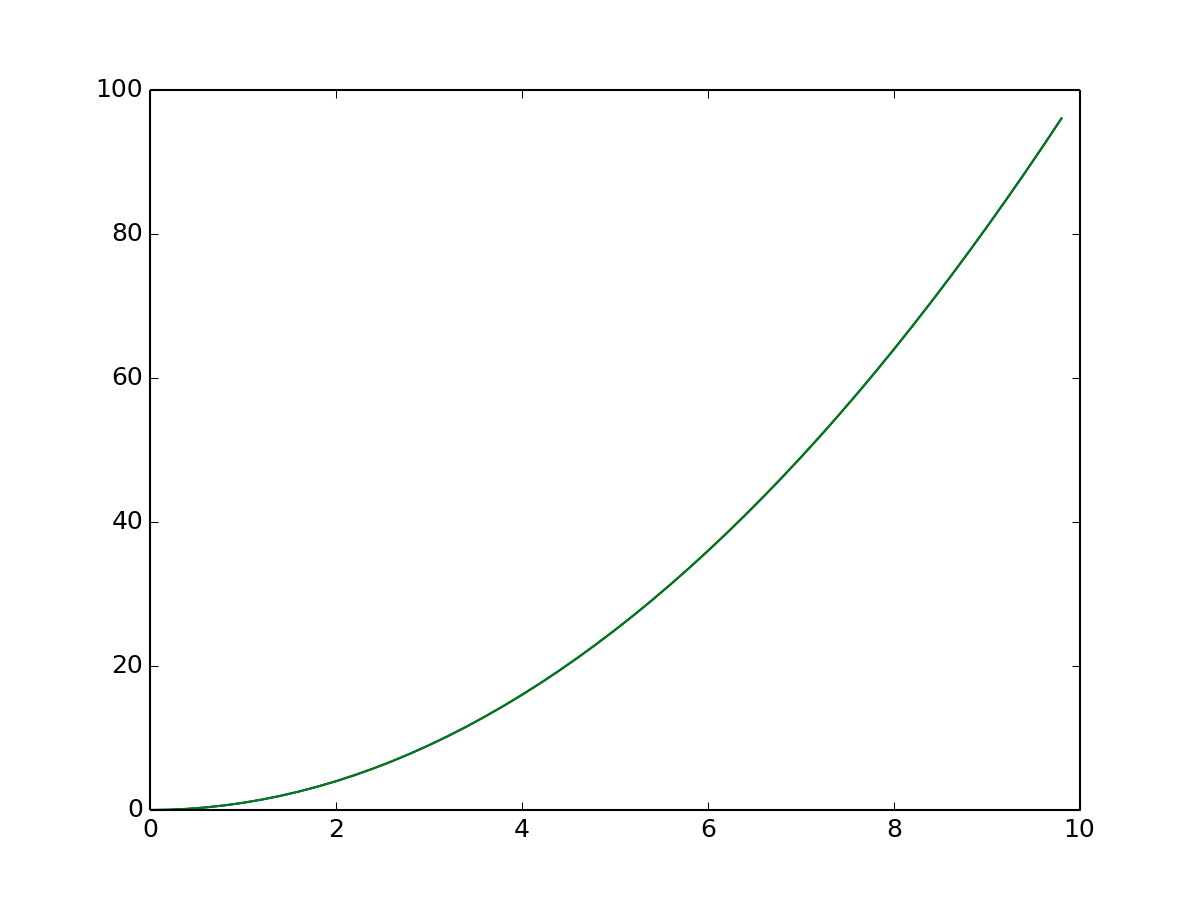
\includegraphics[width=10cm]{plot.png}
\end{minipage}

(opt.: {\tt \%matplotlib inline})

Lit.: 

\begin{itemize}
\item \url{http://matplotlib.org}
\item \url{https://matplotlib.org/faq/usage_faq.html}
\end{itemize}


\item SciPy

\begin{verbatim}
>>> import scipy
\end{verbatim}

Lit.: \url{http://www.scipy.org}


\item Imports for numerical programs (keep namespaces separate!):

\begin{verbatim}
import numpy as np
import matplotlib.pyplot as plt
import scipy
\end{verbatim}

\end{itemize}




\bigskip
{\LARGE\bf TOOLS}
\addcontentsline{toc}{section}{TOOLS} 

\medskip
{\bf Package Distribution}
\addcontentsline{toc}{subsection}{Package Distribution}

\begin{itemize}

\item distutils -- basic support to create and install distributions
  (introduced {\tt setup.py})

\begin{verbatim}
python setup.py --help-commands

build         build_ext       build_py        clean          install 
sdist         upload check    saveopts        bdist          bdist_wheel    
build_sphinx  test            bdist_wininst   [py2exe]       ...
\end{verbatim}

\item setuptools -- enhancements to distutils

   \begin{itemize}
   \item Create wheels with {\tt bdist\_wheels} setuptools extension
   \item Do not use {\tt easy\_install} and {\tt eggs}!
   \end{itemize}

\item wheel -- Binary archive format (successor of {\tt eggs})
      
   \begin{itemize}
   \item {\tt wheel} utility installs and verifies wheels
   \item newer versions of {\tt pip} also work with wheels
   \end{itemize}

\item pip 

   \begin{itemize}

   \item Installs source distributions (sdist/.tar.gz) and binary 
      distributions (wheels/.whl)

   \item Help
   
      \begin{verbatim}
      pip --help, pip install --help

      pip list             list all installed packages
      pip search <str>     Search PyPI for <str>
      pip show <pkg>       show pkg info
      pip install <pkg>    install package
      pip install -U <pkg> upgrade package
      pip uninstall <pkg>  remove packge
      ...
      \end{verbatim}

   \item Trick to choose Python version:
   
      \begin{verbatim}
      python3.6 -m pip install ...   # Linux
      py -3.6 -m pip install ...     # Windows
      \end{verbatim}

   \end{itemize}

   \item Use {\tt twine} to interact with PyPI.

   \item \url{http://www.pyinstaller.org} freezes programs into standalone
         executables on Windows.

\end{itemize}

Lit.: [9]

\label{ipython-section}

\medskip
{\bf IPython}
\addcontentsline{toc}{subsection}{IPython}

Get help with {\tt ?} or {\tt ??} after module, function, 
object, identifier.

\begin{verbatim}
import os
os?
id?
\end{verbatim}

Press {\tt TAB} key to auto-complete.

Commandline arguments

\begin{verbatim}
ipython --help
ipython locate                  # ~/.ipython/
ipython profile help    
ipython profile list
ipython profile create <name>   
ipython --pylab                 # Using matplotlib backend: Qt5Agg (default)
ipython --pylab=tk              # Using matplotlib backend: tk
ipython --matplotlib tk
ipython --matplotlib qt
ipython --profile=hubert        # Start ipython with profile "hubert"
\end{verbatim}

Module {\tt IPython}: {\tt import IPython; print(IPython.version\_info)}

Default config file {\tt ~/.ipython/profile\_default/ipython\_config.py}

Put startup code here: {\tt c.InteractiveShellApp.exec\_lines = "..."}


\medskip
{\bf Ipython Magic}

\setlength{\columnsep}{1cm}
\begin{multicols}{3}

Enter {\tt quickref} or {\tt lsmagic} for a list of magic commands.


{\tt \%quickref} \rval IPy quick reference

{\tt <magic>? \rval help}

{\tt !ls} \rval system command; {\tt L = !ls} store output in list L

In Prompt: {\tt In [26]:}, {\tt \_i26}, {\tt \_ih[26]}, {\tt \_ih[26:27]}

Out Prompt: {\tt Out [26]:}, {\tt \_26}, {\tt \_oh[26]} 

Last 3 Inputs {\tt \_i}, {\tt \_ii}, {\tt \_iii}

Last 3 Outputs {\tt \_}, {\tt \_\_}, {\tt \_\_\_} 

{\tt \#\%\%} \rval cell

{\tt \%<magic>} \rval line magic; {\tt \%\%<magic>} \rval cell magic

{\tt \%bookmark}

{\tt \%cd-<nr>}

{\tt \%cd \~{}}

{\tt \%clear} \rval Konsole löschen

{\tt \%dhist}

{\tt \%dirs}, {\tt \%pushd}, {\tt popd} \rval directory stack

{\tt \%edit}, {\tt \%ed} start editor (env var EDITOR)

{\tt \%env}

{\tt \%exec \_i4}

{\tt \%exit}

{\tt \%history}, {\tt \%hist}

{\tt \%load\_ext [extension]}

Example: automatic module reload

\begin{verbatim}
In [1]: load_ext autoreload
In [2]: autoreload 2
\end{verbatim}

{\tt \%logstart [logfile]}  create log

{\tt \%logstop} close log

{\tt \%logon} temporary on

{\tt \%logoff} temporary off

{\tt \%lsmagic} \rval list available magics

{\tt \%matplotlib} query mpl backend

{\tt \%matplotlib -{}-list} show mpl backends

{\tt \%matplotlib gui} set mpl backend to gui

{\tt \%paste}, {\tt cpaste}

{\tt \%pdb} Control debugger activation

{\tt \%prun} Python code profiler

{\tt \%pycat}

{\tt \%pylab}

{\tt \%pwd}

{\tt \%reset} \rval reset namespace

{\tt \%save}

{\tt \%rep \_i4} \rval edit input line

{\tt \%run pgm.py} \rval run program

{\tt \%run -t pgm.py} \rval report timing

{\tt \%run -d -b<line> pgm.py} \rval debug, set breakpoint at line

{\tt \%run -d -b <file.py>:<line> pgm.py}

{\tt \%time}, {\tt \%timeit}

{\tt \%who}, {\tt \%who\_ls}, {\tt whos}

{\tt \%xdel} delete a variable

{\tt \%xmode}

\end{multicols}

\medskip




\medskip
{\bf Jupyter}
\addcontentsline{toc}{subsection}{Jupyter}

\begin{verbatim}
jupyter --help
jupyter --paths
jupyter <subcommand> --help
jupyter qtconsole --generate-config  # ~/.jupyter/jupyter_qtconsole_config.py
jupyter notebook     # start notebook server
jupyter nbconvert    
\end{verbatim}

Edit {\tt jupyter\_qtconsole\_config.py} to change settings, e.g. font size.

{\tt jupyter nbconvert} can export to serveral formats, e.g. asciidoc, html,
latex, markdown, rst, pdf.

\medskip

{\bf Jupyter notebook keyoard shortcuts}

Command mode (press Esc to enable)

\begin{verbatim}      
Enter edit mode    Enter
Run cell           Sh-Enter
Run cell, ins bel  Alt-Enter
To code            Y
To markdown        M
To raw             R
To heading 1       1
Save + checkpoint  Ctrl-S
Toggle line nmb    L
Toggle output      O
Close pager        ESC
Shortcut help      H
Interrupt kernel   I,I
Restart kernel     0,0
Scroll down        Space
Scroll up          Sh-Space
\end{verbatim}      

Edit mode (press Enter to enable)

\begin{verbatim}      
Code completion    Tab
Tooltip            Sh-Tab
Indent             Ctrl-]
Dedent             Ctrl-[
Select all         Ctrl-A
Undo               Ctrl-Z
Toggle comment     Ctrl-/
\end{verbatim}      


\medskip
{\bf Conda/Pip Package Management}
\addcontentsline{toc}{subsection}{Conda/Pip Package Management}

\begin{verbatim}
--------Conda--------------              --------Pip-------------------
conda 
conda search <package>                   pip search <package>

conda install <package>                  pip install <package>
                                         pip install -U <package>    # Upgrade
conda install python=x.x  
conda install --channel <name> <module>
conda install --name env  scipy

conda list --name <env>                  pip list
conda list --export                      pip freeze
conda install python=x.x
conda update python *
conda install pip                        pip install conda
conda remove <package>                   pip uninstall <package>
conda remove --name <env> <package>
                                         pip show conda
\end{verbatim}

Lit.: https://conda.io/projects/conda/en/latest/user-guide/tasks/

\medskip

{\bf Conda Misc}

Anaconda Prompt Starter (Windows)

\begin{verbatim}
conda update menuinst
conda install -f console_shortcut
\end{verbatim}

Install Mingw Compiler (only for external
programs)

\begin{verbatim}
conda install -c anaconda mingw
\end{verbatim}


Lit.: [10]


\medskip
{\bf Virtual Environments}
\addcontentsline{toc}{subsection}{Virtual Environments}

--- Venv Environments ---

The {\tt pyvenv} tool introduced in Py 3.x is deprecated in 3.6.

\begin{verbatim}
------Linux-------------------         ----------Windows-----------------
python3 -m venv new_env                # py -3.6 -m venv new_env 
source new_env/bin/activate            # new_env\Scripts\activate.bat 
...
deactivate
\end{verbatim}

Delete a virtual env by deactivating and removing the directory.


--- Conda Environments ---

\begin{verbatim}
-----------Linux------------------        -----------Windows----------------
conda create --name <env> pgm[=rev] ...         
conda info --envs (list all envs)        
source activate <env>                     activate <env>
new: conda activate <env>
source deactivate                         deactivate
new: conda deactivate
conda remove --name myenv --all

conda list -e > pkgfile
conda create -n <env> --file < pkgfile
                                         
conda env --help   # modern env
conda env export > pkgfile 
conda env create -f=pkgfile -n <name>
\end{verbatim}

Example: Create environment {\tt testenv} (Linux)

\begin{verbatim}
   $ conda create --name testenv python=3.6
   $ conda activate testenv
   (testenv) hhoegl@e3:~$ _      # ~/miniconda3/envs/testenv/
\end{verbatim}

Example: Create environment {\tt env\_full} with all pkgs in Anaconda (Linux)

\begin{verbatim}
  $ conda create --name env_full anaconda
\end{verbatim}

See pkgs at https://docs.anaconda.com/anaconda/packages/pkg-docs/



Lit.: [10]


\medskip
{\bf Ipdb}
\addcontentsline{toc}{subsection}{Ipdb}

\begin{itemize}
\item {\tt \$ pip install ipdb}

\item 
   \begin{verbatim}
   $ python pgm.py

   # - pgm.py -
   import ipdb
   ...
   ipdb.set_trace()
   \end{verbatim}

\item {\tt ipdb pgm.py \ \ \ \ \  \# or ipdb3}

\item {\tt ipython -{}-pdb pgm.py}

\end{itemize}


\begin{verbatim}
ipdb> help

Documented commands (type help <topic>):
========================================
EOF    cl         disable  interact  next    psource  rv         unt
a      clear      display  j         p       q        s          until
alias  commands   down     jump      pdef    quit     source     up
args   condition  enable   l         pdoc    r        step       w
b      cont       exit     list      pfile   restart  tbreak     whatis
break  continue   h        ll        pinfo   return   u          where
bt     d          help     longlist  pinfo2  retval   unalias
c      debug      ignore   n         pp      run      undisplay
\end{verbatim}


\medskip
{\bf Spyder}
\addcontentsline{toc}{subsection}{Spyder}

{\bf Spyder keyboard shortcuts}

\begin{verbatim}
Quit           C-Q          Go to def      C-G
Restart        A-Sh-R       Find text      C-F
Run            F5           Find next      F3
Fullscreen     F11          Code complete  C-Space
Breakpoint     F12          Undo           C-Z
Debug          C-F5         Indent         Tab
Block comment  C-4          Unindent       Sh-Tab
Block uncomm   C-5          many more, see Tools -> Preferences menu in Spyder
\end{verbatim}      


\medskip

{\bf Windows}
\addcontentsline{toc}{subsection}{Windows}


\begin{tabbing}
    xxxxxxxxxxxxx \= xxxxxxxxxxxxxxxxxxxxxxx \kill
    Ctrl-Sh-ESC   \> Task Manager \\
    Win-R         \> Programm ausführen \\
    Win-Pause     \> Systemeigenschaften \\
    Win-E         \> Explorer \\
    Win-D         \> Desktop  \\
    Ctrl-F        \> Search  \\
\end{tabbing}

\medskip


\addcontentsline{toc}{section}{Literature}
\bibliographystyle{plain}


\begin{thebibliography}{zzzz}

\bibitem{1} Non-Programmer's Tutorial for Python 3

   \url{https://en.wikibooks.org/wiki/Non-Programmer%27s_Tutorial_for_Python_3}

\bibitem{2} Bernd Klein, \url{http://python-kurs.eu}

\bibitem{3} Swaroop C H, A Byte of Python, \url{https://python.swaroopch.com}

\bibitem{4} Mark Pilgrim, Dive Into Python 3

    \url{http://www.diveintopython3.net}

\bibitem{5} Unicode HOWTO

    \url{https://docs.python.org/3/howto/unicode.html}

\bibitem{6} Python 3 Standard Documentation

    \url{https://docs.python.org/3}

\bibitem{7} Michael Weigend, Python ge-packt. 7. Auflage, mitp Verlag, 2018.

\bibitem{8} David Beazley, Python Essential Reference, Addison-Wesley 2009.

\bibitem{9} Python Packaging User Guide

    \url{https://packaging.python.org}

\bibitem{10} Conda Documentation

    \url{https://conda.io/projects/conda/en/latest/index.html}

\end{thebibliography}


\newpage

Your notes:

\newpage

Your notes:

\newpage

Your notes:


% END




\begin{comment}

\newpage % ----------------------------------------------------------------
% Weglassen

\bigskip
{\LARGE\bf Interne Namen}

{\bf Integer}

% IPython help ({\tt i.\_\_<tab>})

\begin{verbatim}
i.__abs__           i.__floordiv__      i.__lt__            i.__reduce_ex__     i.__rxor__
i.__add__           i.__format__        i.__mod__           i.__repr__          i.__setattr__
i.__and__           i.__ge__            i.__mul__           i.__rfloordiv__     i.__sizeof__
i.__bool__          i.__getattribute__  i.__ne__            i.__rlshift__       i.__str__
i.__ceil__          i.__getnewargs__    i.__neg__           i.__rmod__          i.__sub__
i.__class__         i.__gt__            i.__new__           i.__rmul__          i.__subclasshook__
i.__delattr__       i.__hash__          i.__or__            i.__ror__           i.__truediv__
i.__dir__           i.__index__         i.__pos__           i.__round__         i.__trunc__
i.__divmod__        i.__init__          i.__pow__           i.__rpow__          i.__xor__
i.__doc__           i.__int__           i.__radd__          i.__rrshift__       
i.__eq__            i.__invert__        i.__rand__          i.__rshift__        
i.__float__         i.__le__            i.__rdivmod__       i.__rsub__          
i.__floor__         i.__lshift__        i.__reduce__        i.__rtruediv__      
\end{verbatim}

{\bf Float}

\begin{verbatim}
f.__abs__           f.__floordiv__      f.__le__            f.__rdivmod__       f.__rtruediv__
f.__add__           f.__format__        f.__lt__            f.__reduce__        f.__setattr__
f.__bool__          f.__ge__            f.__mod__           f.__reduce_ex__     f.__setformat__
f.__class__         f.__getattribute__  f.__mul__           f.__repr__          f.__sizeof__
f.__delattr__       f.__getformat__     f.__ne__            f.__rfloordiv__     f.__str__
f.__dir__           f.__getnewargs__    f.__neg__           f.__rmod__          f.__sub__
f.__divmod__        f.__gt__            f.__new__           f.__rmul__          f.__subclasshook__
f.__doc__           f.__hash__          f.__pos__           f.__round__         f.__truediv__
f.__eq__            f.__init__          f.__pow__           f.__rpow__          f.__trunc__
f.__float__         f.__int__           f.__radd__          f.__rsub__          
\end{verbatim}


{\bf Complex}

\begin{verbatim}
c.__abs__           c.__float__         c.__int__           c.__pow__           c.__rpow__
c.__add__           c.__floordiv__      c.__le__            c.__radd__          c.__rsub__
c.__bool__          c.__format__        c.__lt__            c.__rdivmod__       c.__rtruediv__
c.__class__         c.__ge__            c.__mod__           c.__reduce__        c.__setattr__
c.__delattr__       c.__getattribute__  c.__mul__           c.__reduce_ex__     c.__sizeof__
c.__dir__           c.__getnewargs__    c.__ne__            c.__repr__          c.__str__
c.__divmod__        c.__gt__            c.__neg__           c.__rfloordiv__     c.__sub__
c.__doc__           c.__hash__          c.__new__           c.__rmod__          c.__subclasshook__
c.__eq__            c.__init__          c.__pos__           c.__rmul__          c.__truediv__
\end{verbatim}


{\bf Strings}

IPython help ({\tt s.\_\_<tab>})

\begin{verbatim}
s.__add__           s.__format__        s.__init__          s.__ne__            s.__setattr__
s.__class__         s.__ge__            s.__iter__          s.__new__           s.__sizeof__
s.__contains__      s.__getattribute__  s.__le__            s.__reduce__        s.__str__
s.__delattr__       s.__getitem__       s.__len__           s.__reduce_ex__     s.__subclasshook__
s.__dir__           s.__getnewargs__    s.__lt__            s.__repr__          
s.__doc__           s.__gt__            s.__mod__           s.__rmod__          
s.__eq__            s.__hash__          s.__mul__           s.__rmul__          
\end{verbatim}


{\bf Tuple}

\begin{verbatim}
T.__add__           T.__eq__            T.__gt__            T.__lt__            T.__repr__
T.__class__         T.__format__        T.__hash__          T.__mul__           T.__rmul__
T.__contains__      T.__ge__            T.__init__          T.__ne__            T.__setattr__
T.__delattr__       T.__getattribute__  T.__iter__          T.__new__           T.__sizeof__
T.__dir__           T.__getitem__       T.__le__            T.__reduce__        T.__str__
T.__doc__           T.__getnewargs__    T.__len__           T.__reduce_ex__     T.__subclasshook__
\end{verbatim}


{\bf List}

IPython: {\tt L.\_\_<tab>}

\begin{verbatim}
L.__add__           L.__eq__            L.__iadd__          L.__mul__           L.__rmul__
L.__class__         L.__format__        L.__imul__          L.__ne__            L.__setattr__
L.__contains__      L.__ge__            L.__init__          L.__new__           L.__setitem__
L.__delattr__       L.__getattribute__  L.__iter__          L.__reduce__        L.__sizeof__
L.__delitem__       L.__getitem__       L.__le__            L.__reduce_ex__     L.__str__
L.__dir__           L.__gt__            L.__len__           L.__repr__          L.__subclasshook__
L.__doc__           L.__hash__          L.__lt__            L.__reversed__      
\end{verbatim}


{\bf Dict}

IPython: {\tt D.\_\_<tab>}

\begin{verbatim}
D.__class__         D.__eq__            D.__hash__          D.__ne__            D.__setitem__
D.__contains__      D.__format__        D.__init__          D.__new__           D.__sizeof__
D.__delattr__       D.__ge__            D.__iter__          D.__reduce__        D.__str__
D.__delitem__       D.__getattribute__  D.__le__            D.__reduce_ex__     D.__subclasshook__
D.__dir__           D.__getitem__       D.__len__           D.__repr__          
D.__doc__           D.__gt__            D.__lt__            D.__setattr__       
\end{verbatim}


{\bf Sets}

\begin{verbatim}
S.__and__           S.__ge__            S.__iter__          S.__rand__          S.__sizeof__
S.__class__         S.__getattribute__  S.__ixor__          S.__reduce__        S.__str__
S.__contains__      S.__gt__            S.__le__            S.__reduce_ex__     S.__sub__
S.__delattr__       S.__hash__          S.__len__           S.__repr__          S.__subclasshook__
S.__dir__           S.__iand__          S.__lt__            S.__ror__           S.__xor__
S.__doc__           S.__init__          S.__ne__            S.__rsub__          
S.__eq__            S.__ior__           S.__new__           S.__rxor__          
S.__format__        S.__isub__          S.__or__            S.__setattr__       
\end{verbatim}


{\bf Functions}

IPython: {\tt fcn.\_\_<tab>}

\begin{verbatim}
fcn.__annotations__   fcn.__doc__           fcn.__init__          fcn.__reduce__
fcn.__call__          fcn.__eq__            fcn.__kwdefaults__    fcn.__reduce_ex__
fcn.__class__         fcn.__format__        fcn.__le__            fcn.__repr__
fcn.__closure__       fcn.__ge__            fcn.__lt__            fcn.__setattr__
fcn.__code__          fcn.__get__           fcn.__module__        fcn.__sizeof__
fcn.__defaults__      fcn.__getattribute__  fcn.__name__          fcn.__str__
fcn.__delattr__       fcn.__globals__       fcn.__ne__            fcn.__subclasshook__
fcn.__dict__          fcn.__gt__            fcn.__new__           
fcn.__dir__           fcn.__hash__          fcn.__qualname__      
\end{verbatim}


{\bf File Objects}

IPython help ({\tt fo.\_\_<tab>})

\begin{verbatim}
fo.__class__         fo.__exit__          fo.__iter__          fo.__repr__
fo.__del__           fo.__format__        fo.__le__            fo.__setattr__
fo.__delattr__       fo.__ge__            fo.__lt__            fo.__sizeof__
fo.__dict__          fo.__getattribute__  fo.__ne__            fo.__str__
fo.__dir__           fo.__getstate__      fo.__new__           fo.__subclasshook__
fo.__doc__           fo.__gt__            fo.__next__          
fo.__enter__         fo.__hash__          fo.__reduce__        
fo.__eq__            fo.__init__          fo.__reduce_ex__     
\end{verbatim}


{\bf Objekte}

IPython help ({\tt obj.\_\_<tab>})

\begin{verbatim}
obj.__class__         obj.__ge__            obj.__module__        obj.__sizeof__
obj.__delattr__       obj.__getattribute__  obj.__ne__            obj.__str__
obj.__dict__          obj.__gt__            obj.__new__           obj.__subclasshook__
obj.__dir__           obj.__hash__          obj.__reduce__        obj.__weakref__
obj.__doc__           obj.__init__          obj.__reduce_ex__     
obj.__eq__            obj.__le__            obj.__repr__          
obj.__format__        obj.__lt__            obj.__setattr__       
\end{verbatim}

\end{comment}


\end{document}

% vim: et sw=4 ts=4
